% Options for packages loaded elsewhere
\PassOptionsToPackage{unicode}{hyperref}
\PassOptionsToPackage{hyphens}{url}
%
\documentclass[
]{book}
\usepackage{lmodern}
\usepackage{amssymb,amsmath}
\usepackage{ifxetex,ifluatex}
\ifnum 0\ifxetex 1\fi\ifluatex 1\fi=0 % if pdftex
  \usepackage[T1]{fontenc}
  \usepackage[utf8]{inputenc}
  \usepackage{textcomp} % provide euro and other symbols
\else % if luatex or xetex
  \usepackage{unicode-math}
  \defaultfontfeatures{Scale=MatchLowercase}
  \defaultfontfeatures[\rmfamily]{Ligatures=TeX,Scale=1}
\fi
% Use upquote if available, for straight quotes in verbatim environments
\IfFileExists{upquote.sty}{\usepackage{upquote}}{}
\IfFileExists{microtype.sty}{% use microtype if available
  \usepackage[]{microtype}
  \UseMicrotypeSet[protrusion]{basicmath} % disable protrusion for tt fonts
}{}
\makeatletter
\@ifundefined{KOMAClassName}{% if non-KOMA class
  \IfFileExists{parskip.sty}{%
    \usepackage{parskip}
  }{% else
    \setlength{\parindent}{0pt}
    \setlength{\parskip}{6pt plus 2pt minus 1pt}}
}{% if KOMA class
  \KOMAoptions{parskip=half}}
\makeatother
\usepackage{xcolor}
\IfFileExists{xurl.sty}{\usepackage{xurl}}{} % add URL line breaks if available
\IfFileExists{bookmark.sty}{\usepackage{bookmark}}{\usepackage{hyperref}}
\hypersetup{
  pdftitle={Statistics and Forensic Science},
  pdfauthor={Jeff Holt},
  hidelinks,
  pdfcreator={LaTeX via pandoc}}
\urlstyle{same} % disable monospaced font for URLs
\usepackage{color}
\usepackage{fancyvrb}
\newcommand{\VerbBar}{|}
\newcommand{\VERB}{\Verb[commandchars=\\\{\}]}
\DefineVerbatimEnvironment{Highlighting}{Verbatim}{commandchars=\\\{\}}
% Add ',fontsize=\small' for more characters per line
\usepackage{framed}
\definecolor{shadecolor}{RGB}{248,248,248}
\newenvironment{Shaded}{\begin{snugshade}}{\end{snugshade}}
\newcommand{\AlertTok}[1]{\textcolor[rgb]{0.94,0.16,0.16}{#1}}
\newcommand{\AnnotationTok}[1]{\textcolor[rgb]{0.56,0.35,0.01}{\textbf{\textit{#1}}}}
\newcommand{\AttributeTok}[1]{\textcolor[rgb]{0.77,0.63,0.00}{#1}}
\newcommand{\BaseNTok}[1]{\textcolor[rgb]{0.00,0.00,0.81}{#1}}
\newcommand{\BuiltInTok}[1]{#1}
\newcommand{\CharTok}[1]{\textcolor[rgb]{0.31,0.60,0.02}{#1}}
\newcommand{\CommentTok}[1]{\textcolor[rgb]{0.56,0.35,0.01}{\textit{#1}}}
\newcommand{\CommentVarTok}[1]{\textcolor[rgb]{0.56,0.35,0.01}{\textbf{\textit{#1}}}}
\newcommand{\ConstantTok}[1]{\textcolor[rgb]{0.00,0.00,0.00}{#1}}
\newcommand{\ControlFlowTok}[1]{\textcolor[rgb]{0.13,0.29,0.53}{\textbf{#1}}}
\newcommand{\DataTypeTok}[1]{\textcolor[rgb]{0.13,0.29,0.53}{#1}}
\newcommand{\DecValTok}[1]{\textcolor[rgb]{0.00,0.00,0.81}{#1}}
\newcommand{\DocumentationTok}[1]{\textcolor[rgb]{0.56,0.35,0.01}{\textbf{\textit{#1}}}}
\newcommand{\ErrorTok}[1]{\textcolor[rgb]{0.64,0.00,0.00}{\textbf{#1}}}
\newcommand{\ExtensionTok}[1]{#1}
\newcommand{\FloatTok}[1]{\textcolor[rgb]{0.00,0.00,0.81}{#1}}
\newcommand{\FunctionTok}[1]{\textcolor[rgb]{0.00,0.00,0.00}{#1}}
\newcommand{\ImportTok}[1]{#1}
\newcommand{\InformationTok}[1]{\textcolor[rgb]{0.56,0.35,0.01}{\textbf{\textit{#1}}}}
\newcommand{\KeywordTok}[1]{\textcolor[rgb]{0.13,0.29,0.53}{\textbf{#1}}}
\newcommand{\NormalTok}[1]{#1}
\newcommand{\OperatorTok}[1]{\textcolor[rgb]{0.81,0.36,0.00}{\textbf{#1}}}
\newcommand{\OtherTok}[1]{\textcolor[rgb]{0.56,0.35,0.01}{#1}}
\newcommand{\PreprocessorTok}[1]{\textcolor[rgb]{0.56,0.35,0.01}{\textit{#1}}}
\newcommand{\RegionMarkerTok}[1]{#1}
\newcommand{\SpecialCharTok}[1]{\textcolor[rgb]{0.00,0.00,0.00}{#1}}
\newcommand{\SpecialStringTok}[1]{\textcolor[rgb]{0.31,0.60,0.02}{#1}}
\newcommand{\StringTok}[1]{\textcolor[rgb]{0.31,0.60,0.02}{#1}}
\newcommand{\VariableTok}[1]{\textcolor[rgb]{0.00,0.00,0.00}{#1}}
\newcommand{\VerbatimStringTok}[1]{\textcolor[rgb]{0.31,0.60,0.02}{#1}}
\newcommand{\WarningTok}[1]{\textcolor[rgb]{0.56,0.35,0.01}{\textbf{\textit{#1}}}}
\usepackage{longtable,booktabs}
% Correct order of tables after \paragraph or \subparagraph
\usepackage{etoolbox}
\makeatletter
\patchcmd\longtable{\par}{\if@noskipsec\mbox{}\fi\par}{}{}
\makeatother
% Allow footnotes in longtable head/foot
\IfFileExists{footnotehyper.sty}{\usepackage{footnotehyper}}{\usepackage{footnote}}
\makesavenoteenv{longtable}
\usepackage{graphicx,grffile}
\makeatletter
\def\maxwidth{\ifdim\Gin@nat@width>\linewidth\linewidth\else\Gin@nat@width\fi}
\def\maxheight{\ifdim\Gin@nat@height>\textheight\textheight\else\Gin@nat@height\fi}
\makeatother
% Scale images if necessary, so that they will not overflow the page
% margins by default, and it is still possible to overwrite the defaults
% using explicit options in \includegraphics[width, height, ...]{}
\setkeys{Gin}{width=\maxwidth,height=\maxheight,keepaspectratio}
% Set default figure placement to htbp
\makeatletter
\def\fps@figure{htbp}
\makeatother
\setlength{\emergencystretch}{3em} % prevent overfull lines
\providecommand{\tightlist}{%
  \setlength{\itemsep}{0pt}\setlength{\parskip}{0pt}}
\setcounter{secnumdepth}{5}
\usepackage{booktabs}
\usepackage{amsthm}
\makeatletter
\def\thm@space@setup{%
  \thm@preskip=8pt plus 2pt minus 4pt
  \thm@postskip=\thm@preskip
}
\makeatother
\usepackage[]{natbib}
\bibliographystyle{apalike}

\title{Statistics and Forensic Science}
\author{Jeff Holt}
\date{2021-12-20}

\begin{document}
\maketitle

{
\setcounter{tocdepth}{1}
\tableofcontents
}
\hypertarget{prerequisites}{%
\chapter{Prerequisites}\label{prerequisites}}

This is a sample book that is currently a work in progress by the \emph{University of Virginia}. This is not a finished product.

\hypertarget{intro}{%
\chapter{Introduction}\label{intro}}

You can label chapter and section titles using \texttt{\{\#label\}} after them, e.g., we can reference Chapter \ref{intro}. If you do not manually label them, there will be automatic labels anyway, e.g., Chapter \ref{methods}.

Figures and tables with captions will be placed in \texttt{figure} and \texttt{table} environments, respectively.

\begin{Shaded}
\begin{Highlighting}[]
\KeywordTok{par}\NormalTok{(}\DataTypeTok{mar =} \KeywordTok{c}\NormalTok{(}\DecValTok{4}\NormalTok{, }\DecValTok{4}\NormalTok{, }\FloatTok{.1}\NormalTok{, }\FloatTok{.1}\NormalTok{))}
\KeywordTok{plot}\NormalTok{(pressure, }\DataTypeTok{type =} \StringTok{'b'}\NormalTok{, }\DataTypeTok{pch =} \DecValTok{19}\NormalTok{)}
\end{Highlighting}
\end{Shaded}

\begin{figure}

{\centering 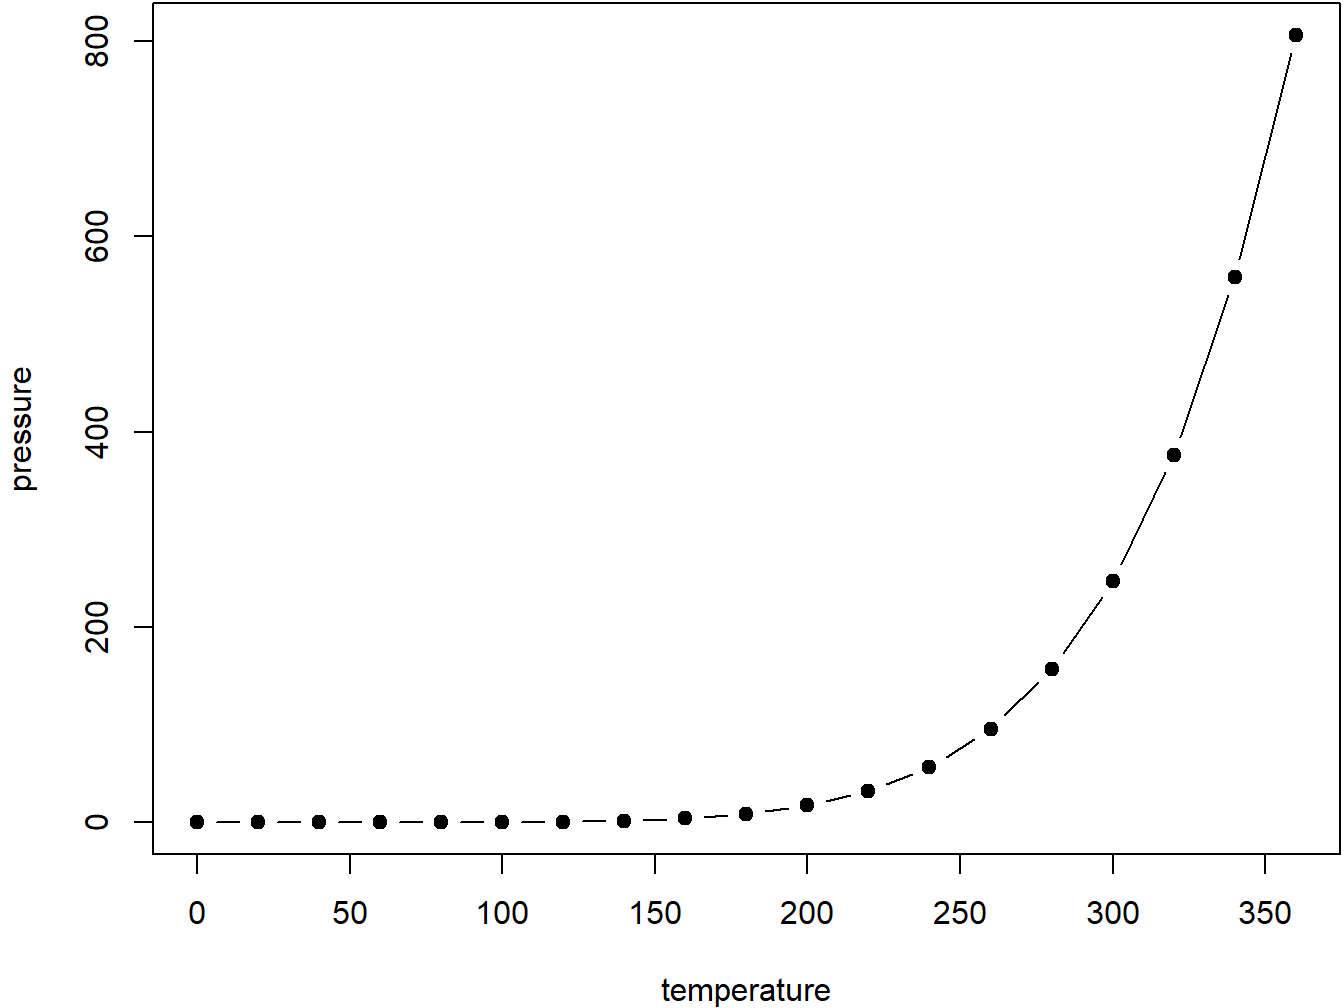
\includegraphics[width=0.8\linewidth]{bookdown-demo_files/figure-latex/nice-fig-1} 

}

\caption{Here is a nice figure!}\label{fig:nice-fig}
\end{figure}

Reference a figure by its code chunk label with the \texttt{fig:} prefix, e.g., see Figure \ref{fig:nice-fig}. Similarly, you can reference tables generated from \texttt{knitr::kable()}, e.g., see Table \ref{tab:nice-tab}.

\begin{Shaded}
\begin{Highlighting}[]
\NormalTok{knitr}\OperatorTok{::}\KeywordTok{kable}\NormalTok{(}
  \KeywordTok{head}\NormalTok{(iris, }\DecValTok{20}\NormalTok{), }\DataTypeTok{caption =} \StringTok{'Here is a nice table!'}\NormalTok{,}
  \DataTypeTok{booktabs =} \OtherTok{TRUE}
\NormalTok{)}
\end{Highlighting}
\end{Shaded}

\begin{table}

\caption{\label{tab:nice-tab}Here is a nice table!}
\centering
\begin{tabular}[t]{rrrrl}
\toprule
Sepal.Length & Sepal.Width & Petal.Length & Petal.Width & Species\\
\midrule
5.1 & 3.5 & 1.4 & 0.2 & setosa\\
4.9 & 3.0 & 1.4 & 0.2 & setosa\\
4.7 & 3.2 & 1.3 & 0.2 & setosa\\
4.6 & 3.1 & 1.5 & 0.2 & setosa\\
5.0 & 3.6 & 1.4 & 0.2 & setosa\\
\addlinespace
5.4 & 3.9 & 1.7 & 0.4 & setosa\\
4.6 & 3.4 & 1.4 & 0.3 & setosa\\
5.0 & 3.4 & 1.5 & 0.2 & setosa\\
4.4 & 2.9 & 1.4 & 0.2 & setosa\\
4.9 & 3.1 & 1.5 & 0.1 & setosa\\
\addlinespace
5.4 & 3.7 & 1.5 & 0.2 & setosa\\
4.8 & 3.4 & 1.6 & 0.2 & setosa\\
4.8 & 3.0 & 1.4 & 0.1 & setosa\\
4.3 & 3.0 & 1.1 & 0.1 & setosa\\
5.8 & 4.0 & 1.2 & 0.2 & setosa\\
\addlinespace
5.7 & 4.4 & 1.5 & 0.4 & setosa\\
5.4 & 3.9 & 1.3 & 0.4 & setosa\\
5.1 & 3.5 & 1.4 & 0.3 & setosa\\
5.7 & 3.8 & 1.7 & 0.3 & setosa\\
5.1 & 3.8 & 1.5 & 0.3 & setosa\\
\bottomrule
\end{tabular}
\end{table}

You can write citations, too. For example, we are using the \textbf{bookdown} package \citep{R-bookdown} in this sample book, which was built on top of R Markdown and \textbf{knitr} \citep{xie2015}.

\hypertarget{literature}{%
\chapter{Literature}\label{literature}}

Here is a review of existing methods.

\hypertarget{probability}{%
\chapter{Probability}\label{probability}}

Probability is an important and complex field of study. Fortunately, only a few basic issues in probability theory are essential for understanding statistics at the level covered in this book. These basic issues are covered in this chapter.

\hypertarget{introduction}{%
\section{Introduction}\label{introduction}}

TODO: Edit the introductory section below.

\emph{``The introductory section discusses the definitions of probability. This is not as simple as it may seem. The section on basic concepts covers how to compute probabilities in a variety of simple situations. The Gambler's Fallacy Simulation provides an opportunity to explore this fallacy by simulation. The Birthday Demonstration illustrates the probability of finding two or more people with the same birthday. The Binomial Demonstration shows the binomial distribution for different parameters. The section on base rates discusses an important but often-ignored factor in determining probabilities. It also presents Bayes' Theorem. The Bayes' Theorem Demonstration shows how a tree diagram and Bayes' Theorem result in the same answer. Finally, the Monty Hall Demonstration lets you play a game with a very counterintuitive result.''}

\hypertarget{another-subsection}{%
\section{Another Subsection}\label{another-subsection}}

In what follows we introduce the basics of probability, which quantifies the
chance that something occurs. Let's start with a specific situation to serve
as an example. Suppose that we have a population of 1000 people, each classified
by gender (Female or Male) and blood type (A, AB, B, or O). The number of
people of each combination of gender and blood type is
shown in the table below.

\[
\begin{array}{c|c|c}
           & \mathrm{F} & \mathrm{M}\\ \hline
\mathrm{A} & 175 & 235 \\ 
\mathrm{AB} & 16 & 24 \\ 
\mathrm{B} & 37 & 63 \\ 
\mathrm{O} & 202 & 248 \\ 
\end{array}\\
\mbox{Gender and blood type counts}
\]

Suppose that we select one of the people at random, and note that person's gender and blood type. There are various possibilities for outcomes, such as the person selected is female with Type A blood. The chance that this outcome occurs is called the \textbf{probability} of this outcome. As 175 out
of the 1000 people are female of blood type A, the probability of selecting such a person is

\[\mbox{P(Female and Type A)} = \frac{175}{1000} = 0.175\]

Here P(Female and Type A) stands for the probability that the person
selected is Female \textbf{and} has Type A blood. A sample of other probabilities
that come directly from the table are

\[
\begin{array}{rcccl}
\mbox{P(Female and Type O)} & = & {\displaystyle\frac{202}{1000}} & = & 0.202 \\[5pt]
\mbox{P(Male and Type AB)} & = & {\displaystyle\frac{24}{1000}} & = & 0.024 \\[5pt]
\mbox{P(Male and Type A)} & = & {\displaystyle\frac{235}{1000}} & = & 0.235 \\
\end{array}
\]

We also can combine table entries to compute other probabilities. For
instance, there are a total of \(235 + 24 + 63 + 248 = 570\) males in
our population, so

\[
\mbox{P(Male)} = \frac{570}{1000} = 0.57
\]

There are a total of \(16 + 24 = 40\) people with blood type AB, so

\[
\mbox{P(Type AB)} = \frac{40}{1000} = 0.04
\]

\hypertarget{sample-questions}{%
\subsection{Sample Questions}\label{sample-questions}}

\textbf{1.} What is the probability that the person selected is female?

\textbf{Answer:} \(P(\text{Female}) = 1 - P(\text{Male}) = 1 - 0.57 = 0.43\) This is equivalent to \((175 + 16 + 37 + 202) / 1000\).

\textbf{2.} What is the probability that the person selected is male and has type A blood and type O blood?

\textbf{Answer:} \(P(\text{Male and A and O}) = 0\). The probability of this event occurring in the table is zero, as no men have two different types of blood.

\hypertarget{and-vs-or}{%
\section{And vs Or}\label{and-vs-or}}

Above we saw that \(\mbox{P(Female and Type A)} = 0.175\). Suppose we
we instead would like to know \(\mbox{P(Female or Type A)}\)? That is,
we want to know the probability that a randomly selected person
is either female or has type A blood. (Note that this group includes those
who are both female \textbf{and} have type A blood.) From our table we see that
the total number in this group is \(175+16+37+202+235 = 665\) so that

\[
\mbox{P(Female or Type A)} = \frac{665}{1000} = 0.665
\]

Other combinations are also possible. For instance, there
are \(175 + 235 = 310\) people with type A blood and
\(37 + 63 = 100\) people with type B blood, so there are a total of
\(310 + 100 = 410\) people that have either type A or type B blood. Therefore, we
have

\[
\mbox{P(Type A or Type B)} = \frac{410}{1000} = 0.41
\]

\hypertarget{sample-questions-1}{%
\subsection{Sample Questions}\label{sample-questions-1}}

\textbf{1.} What is the probability of selecting a female or male with type AB blood?

\textbf{Answer:} \(P(\text{(Male or Female) and AB}) = P(\text{(Male and AB) or (Female and AB)}) = (16 + 24) / 1000 = 0.04\)

\hypertarget{conditional-probability}{%
\section{Conditional Probability}\label{conditional-probability}}

Now suppose that we just focus on the females in the population, which
forms a subset of the population. The probability that a randomly selected
female has blood type O is an example of a \textbf{conditional probability}.

There are 430 females in the population, and 202 of those have type O blood.\\
Hence the probability that female chosen at random has type O blood is

\[
\mbox{P(Type O | Female)} = \frac{202}{430} = 0.470
\]

The notation \(\mbox{P(Type O | Female)}\) is read out loud as
\emph{The probability of blood type O, given the individual is female.}
Conditional probabilities arise all the time when evaluating forensic evidence.
Other examples of conditional probabilities:

The probability of Type AB, given that the person is male:

\[
\mbox{Pr(Type AB | Male)} = \frac{24}{570} = 0.042
\]

The probability the person is female, given Type B blood:

\[
\mbox{Pr(Female | Type B)} = \frac{37}{100} = 0.37
\]
The probability the person is male, given Type A blood:

\[
\mbox{Pr(Male | Type A)} = \frac{235}{410} = 0.573
\]

\hypertarget{sample-questions-2}{%
\subsection{Sample Questions}\label{sample-questions-2}}

\textbf{1.} What is the probability of blood type AB or B given the person selected is female?

\textbf{Answer:} \(P(\text{AB or B | Female}) = (16 + 37) / 430 = 0.123\)

\hypertarget{methods}{%
\chapter{Methods}\label{methods}}

We describe our methods in this chapter.

Math can be added in body using usual syntax like this

\hypertarget{math-example}{%
\section{math example}\label{math-example}}

\(p\) is unknown but expected to be around 1/3. Standard error will be approximated

\[
SE = \sqrt(\frac{p(1-p)}{n}) \approx \sqrt{\frac{1/3 (1 - 1/3)} {300}} = 0.027
\]

You can also use math in footnotes like this\footnote{where we mention \(p = \frac{a}{b}\)}.

We will approximate standard error to 0.027\footnote{\(p\) is unknown but expected to be around 1/3. Standard error will be approximated

  \[
  SE = \sqrt(\frac{p(1-p)}{n}) \approx \sqrt{\frac{1/3 (1 - 1/3)} {300}} = 0.027
  \]}

\hypertarget{applications}{%
\chapter{Applications}\label{applications}}

Some \emph{significant} applications are demonstrated in this chapter.

\hypertarget{example-one}{%
\section{Example one}\label{example-one}}

\hypertarget{example-two}{%
\section{Example two}\label{example-two}}

\hypertarget{final-words}{%
\chapter{Final Words}\label{final-words}}

We have finished a nice book.

  \bibliography{book.bib,packages.bib}

\end{document}
